%  $
% \newcommand{\MtdFull}[1]{\frac{D \, #1}{D \, t}}
% \newcommand{\Pd}[2]{\frac{\partial #1}{\partial #2}}
% \newcommand{\dt}[1]{#1 ^{\bullet}}
% \newcommand{\dV}{\; \text{d}V}
% \newcommand{\dA}{\; \text{d}A}
% \newcommand{\dx}{\; \text{ d}x}
% \newcommand{\dy}{\; \text{ d}y}
% \newcommand{\dz}{\; \text{ d}z}
% \newcommand{\dxi}{\; \text{ d}\xi}
% \newcommand{\deta}{\; \text{ d}\eta}
% \newcommand{\dzeta}{\; \text{ d}\zeta}
% \newcommand{\grad}[1]{\text{grad}\left(#1\right)}
% \renewcommand{\div}[1]{\text{div} \left(#1\right)}
% \newcommand{\td}[1]{\dot{#1}}
% \newcommand{\tdd}[1]{\ddot{#1}}
% \newcommand{\T}{\rp{T}}
% \newcommand{\rp}[1]{^{\text{#1}}}
% \newcommand{\rs}[1]{_{\text{#1}}}
% \renewcommand{\bm}[1]{\boldsymbol{#1}}
% \newcommand{\e}{\epsilon}
% \newcommand{\eb}{\bm{\e}}
% \newcommand{\s}{\sigma}
% \newcommand{\sb}{\bm{\sigma}}
% $

%  ```{admonition} Todo
% :class: warning
% - [x] Motivation
% - [x] Lernziele
% - [x] Bilanzgleichungen
%    - [x] lokale Form 
%    - [x] Randbedingungen
%    - [x] Anwendung
%    - [x] Zusammenfassende Tabelle
% - [x] Kinematik
%    - [x] lineare Kinematik
% - [x] Materialmodellierung
%    - [x] Wärmeleitung nach Fourier
%    - [x] Lineare Elastizität
%    - [x] Ausblick
%    - [x] Ebener Spannungszustand
%    - [x] Ebener Verzerrungszustand
%    - [x] Rotationssymmetrie
% ```

%  -+-+-+-+-+-+-AI-SPLIT

\begin{framed}
\textbf{Lernziele}\\
\begin{itemize}
\item Wie werden mechanische Problemstellungen formuliert?
\item Was sind die Unbekannten der Bilanzgleichungen?
\item Welche Zutaten braucht man, um ein lösbares Problem zu erhalten?
\item Wie lauten die wesentlichen Bilanzgleichungen der Kontinuumsmechanik?
\item In welche Kategorien werden Randbedingungen untergliedert?
\item Wozu brauchen wir Materialmodelle?
\item Welche sind die grundlegenden Materialmodelle der Wärmeleitung, des Fluidtransports und der Strukturmechanik?
\item Mit welchen Vereinfachungen kann die Dimensionalität der Problemstellung reduziert werden?
\item Was sind die Voraussetzungen hierfür?
\end{itemize}
\end{framed}

\subsubsection{Mathematische Modellbildung in der Kontinuumstheorie}

In diesem Kapitel werden die grundlegenden Gleichungen der Kontinuumsmechanik vorgestellt. Dies dient als Ausgangspunkt für die numerische Lösung mechanischer Problemstellungen. Während der Vorstellung der Ausgangsgleichungen wird zudem die verwendete Notation eingeführt.

\paragraph{Notation}

Im Rahmen dieses Moduls wird die folgende symbolische Schreibweise verwendet:

\bigskip\noindent
\begin{tabular}{p{\dimexpr 0.333\linewidth-2\tabcolsep}p{\dimexpr 0.333\linewidth-2\tabcolsep}p{\dimexpr 0.333\linewidth-2\tabcolsep}}
\toprule
Tensorstufe & Symbol & Tensorschreibweise \\
\hline
Tensor der Stufe 0 (Skalar) & $a$, $b$, $\varphi$ & $a$, $b$, $\varphi$ \\
Tensor der Stufe 1 (Vektor) & $\bm{a}$, $\bm{b}$ & $a_i\bm{e}_i$, $b_i\bm{e}_i$ \\
Tensor der Stufe 2 (Dyade) & $\bm{A}$, $\bm{\sigma}$ & $A_{ij}\bm{e}_i\bm{e}_j$, $B_{ij}\bm{e}_i\bm{e}_j$ \\
Tensor der Stufe 4 & $\mathbb{C}$, $\mathbb{A}$ & $\mathbb{C}\bm{e}_i\bm{e}_j\bm{e}_k\bm{e}_l$, $\mathbb{A}\bm{e}_i\bm{e}_j\bm{e}_k\bm{e}_l$ \\
\bottomrule
\end{tabular}

Soweit möglich erhalten Tensoren der Stufe 2 Gro$\beta$buchstaben als Symbol, während Vektoren mit Kleinbuchstaben dargestellt werden. Handschriftlich wird ein Tensor durch einen Unterstrich repräsentiert $\underline{A}=\bm{A}$. Für Vektoren ist alternativ auch der Vektorpfeil gebräuchlich $\underline{a} = \vec{a} = \bm{a}$.

%  -+-+-+-+-+-+-AI-SPLIT

\paragraph{Bilanzgleichungen der Kontinuumsmechanik}

In diesem Abschnitt werden wir die grundlegenden Bilanzgleichungen der Kontinuumsmechanik einführen. Diese Gleichungen sind das Fundament für die Beschreibung des physikalischen Verhaltens und bilden den Ausgangspunkt für die Finite-Elemente-Methode. Die Bilanzgleichungen repräsentieren Erhaltungsprinzipien, die für jedes Kontinuum gelten, unabhängig von den spezifischen Materialeigenschaften. Die Bilanzgleichungen dienen als Bestimmungsgleichung für die Feldgrö$\beta$en:

\begin{itemize}
\item Druck $p(\bm{x},t)$
\item Verschiebung $\bm{u}(\bm{x},t)$
\item Temperatur $\theta(\bm{x},t)$.
\end{itemize}

Als Feldgrö$\beta$e bezeichnet man physikalische Grö$\beta$en, denen zu jedem Zeitpunkt $t$ und zu jedem materiellen Punkt $\bm{x}$ ein Wert zugeordnet wird.

Die vier wesentlichen Bilanzgleichungen sind:

\begin{itemize}
\item Massenerhaltung
\item Impulserhaltung
\item Drehimpulserhaltung (hieraus resultiert die Symmetrie des Spannungstensors $\bm{\sigma}$)
\item Energieerhaltung (1. Hauptsatz der Thermodynamik)
\end{itemize}

\subparagraph{Massenerhaltung}

\begin{figure}[!htbp]
\centering
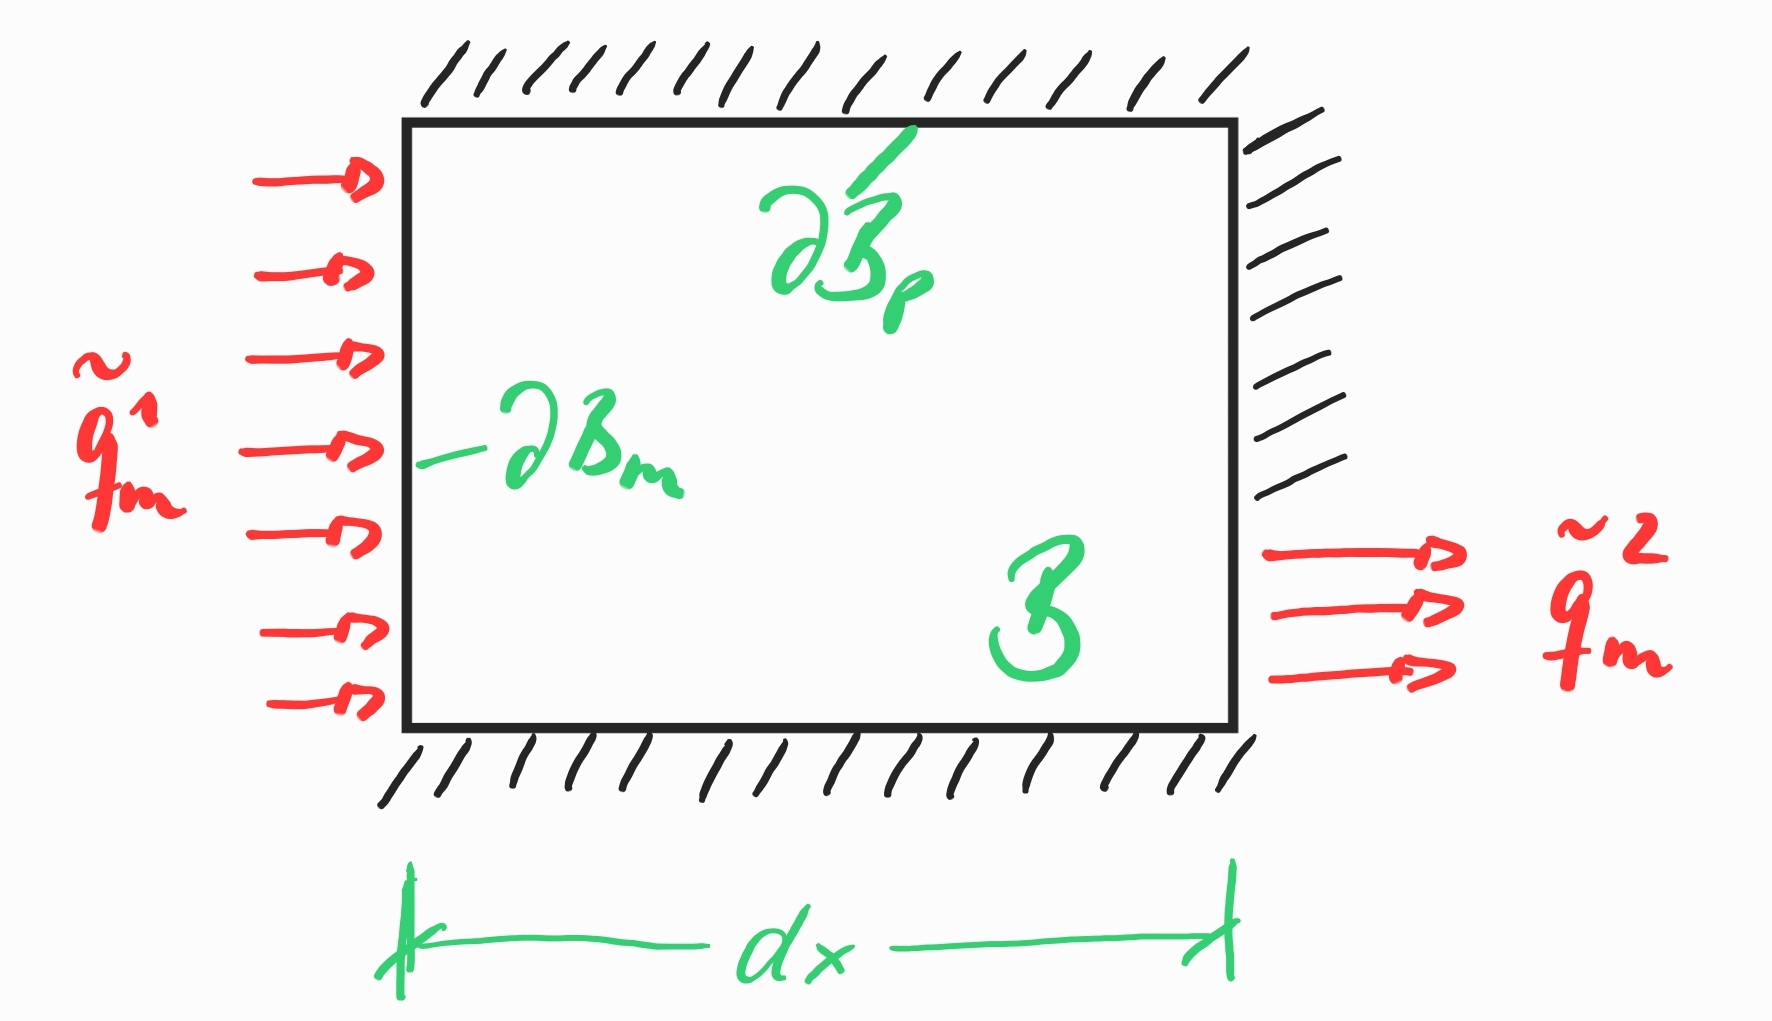
\includegraphics[width=0.7\linewidth]{files/Massenbilanz-5249ed792f311467066a05421a26a64c.jpg}
\caption[]{Ein- und Ausfluss eines infinitesimalen Volumenelementes \textbf{Austausch}}
\label{massenbilanz}
\end{figure}

Die Massenerhaltung besagt, dass die Masse eines geschlossenen Systems konstant bleibt, oder, wie in der Abbildung dargestellt, dass die zeitliche Änderung der Masse eines Systems gleich der Differenz von Zustrom und Abfluss ist. In Abwesenheit von Massenquellen oder -senken kann dies mathematisch ausgedrückt werden als:

\begin{equation}
\label{Massenbilanz}
\dot{\varrho} +  \div{\varrho {\bm{v}}} = 0
\end{equation}

Hier ist $\varrho$ die Dichte und $\bm{v}$ die Geschwindigkeit des Materials. Die zeitliche Ableitung einer Grö$\beta$e $\square$ wird durch einen Punkt über der Grö$\beta$e dargestellt: $\td{\square}$.

\begin{framed}
\textbf{Note}\\
Die Massenbilanz ist für gewöhnliche Festkörper stets erfüllt und muss nicht separat gelöst werden. Anders sieht dies im Bereich der Biomechanik oder Geomechanik aus. Hier gibt es z.B. Wachstumsprozesse (Knochen) oder Sickerströmungen. Mit der Massenbilanz kann man die Konzentration $c(\bm{x},t)$ eines Bestandteils oder den Druck $p(\bm{x},t)$ einer Phase bestimmen.
\end{framed}

Formuliert man die Massenbilanz für Fluide, dann ist die Massendichte eine Funktion des Drucks $p$, und man kann die Zeitableitung in Figure~\ref{Massenbilanz} über die Kettenregel auswerten:

\begin{equation}
\label{Massenbilanz2}
 \underbrace{\Pd{\varrho}{p}}_{=:\frac{\varrho}{\kappa}} \td{p} + \div{\varrho {\bm{v}}} = 0 \; .
\end{equation}

Die primäre Grö$\beta$e, nach der die partielle Differentialgleichung gelöst wird, ist damit der Druck $p$. Als sekundäre Grö$\beta$e bezeichnet man Feldgrö$\beta$en, die von den primären Grö$\beta$en abgeleitet sind. Im Fall der Massenbilanz des Fluids ist dies die Geschwindigkeit der Materialpartikel $\bm{v}$. Die Gleichungen Figure~\ref{Massenbilanz} und (\ref{Massenbilanz2}) beschreiben, wie sich die bilanzierte Grö$\beta$e ($p$) in der Zeit verändert; eine Information über den absoluten Wert der Grö$\beta$e erhält man erst mit der Einführung von Anfangs- und Randwerten:

\begin{align}
p(\bm{x},t=t_0) & = \tilde{p}_0 \qquad &\forall \bm{x} \in \mathcal{B}& \\
p(\bm{x},t) & = \tilde{p} \qquad &\forall \bm{x} \in \partial \mathcal{B}_p& \\
\varrho \bm{v}\T \bm{n} & = \tilde{q}_m \qquad &\forall \bm{x} \in \partial\mathcal{B}_m&
\end{align}

Hierbei wird der zweite Term auch als Dirichlet oder wesentliche Randbedingung und der dritte Term als Neumann oder natürliche Randbedingung bezeichnet.

Diese Art der mathematischen Problemstellung nennt man Anfangsrandwertproblem (IBVP - Initial Boundary Value Problem).

\begin{framed}
\textbf{IVBP1 - Massenerhaltung}\\
Bestimme das Druckfeld $p(\bm{x},t): \mathcal{B} \times [t_0,t] \rightarrow \mathcal{R}^1$, sodass für alle materiellen Punkte $\bm{x} \, \in \, \mathcal{B}$ zu jedem Zeitpunkt $t \, \in \, [t_0,t]$ die Bilanzgleichung:

\begin{equation}
\frac{\varrho}{\kappa} \td{p} + \div{\varrho {\bm{v}}} = 0
\end{equation}

unter Einhaltung der Anfangs- und Randbedingungen:

\begin{align}
p(\bm{x},t=t_0) & = \tilde{p}_0 \qquad &\forall \bm{x} \in \mathcal{B}& \\
p(\bm{x},t) & = \tilde{p} \qquad &\forall \bm{x} \in \partial \mathcal{B}_p& \\
\varrho \bm{v}\T \bm{n} & = \tilde{q}_m \qquad &\forall \bm{x} \in \partial\mathcal{B}_m&
\end{align}

erfüllt ist.
\end{framed}

%  -+-+-+-+-+-+-AI-SPLIT

\subparagraph{Impulserhaltung}

\begin{figure}[!htbp]
\centering
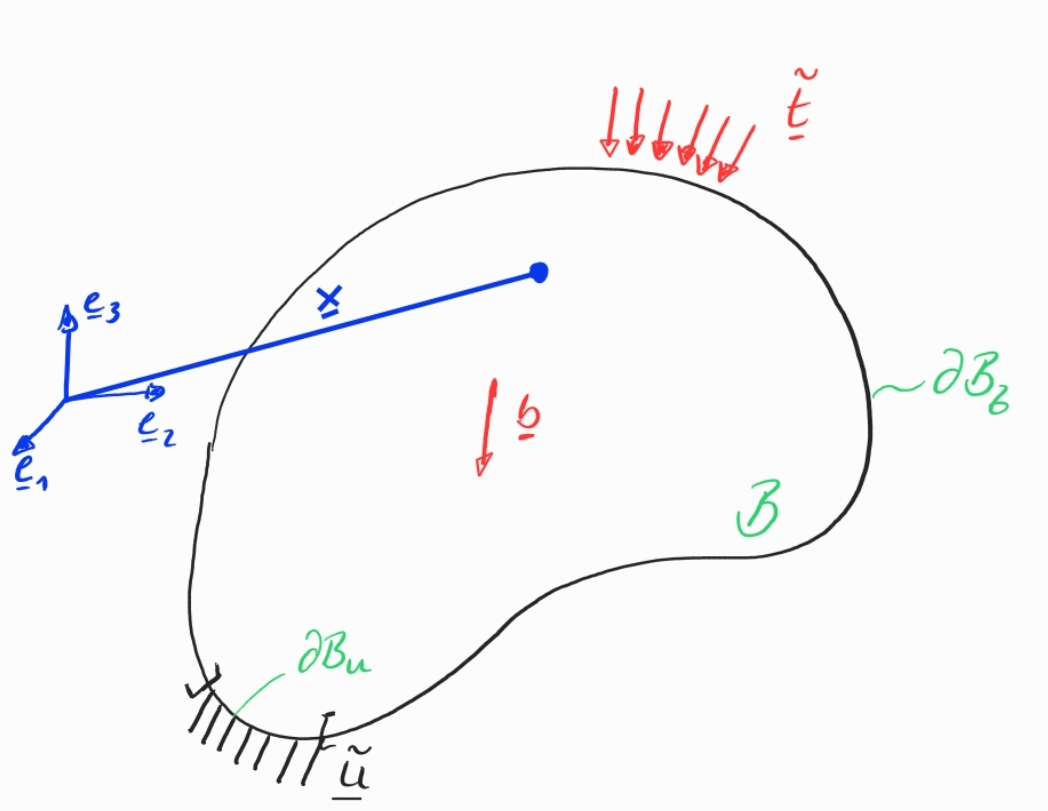
\includegraphics[width=0.7\linewidth]{files/Impulsbilanz-3c1ed32b03eec7db5f7e582ea9b4a7c5.jpg}
\caption[]{Körper $\mathcal{B}$ unter Einwirkung der externen Oberflächenkraft $\tilde{\bm{t}}$ und der Volumenlast $\bm{b}$}
\label{impulsbilanz_fig_1}
\end{figure}

Die Impulserhaltung, oft formuliert als Newtons zweites Gesetz, besagt, dass die Änderung des Impulses $\rho \bm{v}$ eines Körpers gleich der Summe der auf ihn wirkenden Kräfte ist. Für ein Kontinuum wird dies durch die Cauchy-Bewegungsgleichungen ausgedrückt:

\begin{equation}
\varrho \td{\bm{v}} =\div{\bm{\sigma}} + \rho \bm{b}
\end{equation}

$\boldsymbol{\sigma}$ steht hierbei für den Spannungstensor und $\mathbf{b}$ für die Volumenkraft pro Masseneinheit.

\begin{framed}
\textbf{Note}\\
Die Impulsbilanz ist eine vektorielle partielle Differentialgleichung. Mit ihrer Hilfe kann man das Verschiebungsfeld $\bm{u}(\bm{x},t)$ und das Spannungsfeld $\bm{\sigma}(\bm{x},t)$ eines Festkörpers bestimmen.
\end{framed}

Die primäre Feldgrö$\beta$e dieses Anfangsrandwertproblems ist die Verschiebung $\bm{u}(\bm{x},t)$ der Materialpartikel. Die sekundäre Grö$\beta$e ist die Spannung $\bm{\sigma}(\bm{x},t)$, welche wiederum von den Dehnungen $\bm{\epsilon}$ abhängig ist. Als Randwerte können entweder Verschiebungen (wesentliche Randbedingungen) vorgegeben werden oder Oberflächenspannungen (natürliche Randbedingungen).

\begin{framed}
\textbf{IVBP2 - Impulsbilanz}\\
Bestimme das Verschiebungsfeld $\bm{u}(\bm{x},t): \mathcal{B} \times [t_0,t] \rightarrow \mathcal{R}^3$, sodass für alle materiellen Punkte $\bm{x} \, \in \, \mathcal{B}$ zu jedem Zeitpunkt $t \, \in \, [t_0,t]$ die Bilanzgleichung:

\begin{equation}
\varrho \td{\bm{v}} =\div{\bm{\sigma}} + \rho \bm{b}
\end{equation}

unter Einhaltung der Anfangs- und Randbedingungen:

\begin{align}
\bm{u}(\bm{x},t=t_0) & = \tilde{\bm{u}}_0 \qquad &\forall \bm{x} \in \mathcal{B}& \\
\bm{u}(\bm{x},t) & = \tilde{\bm{u}} \qquad &\forall \bm{x} \in \partial \mathcal{B}_u& \\
\bm{\sigma}\T \bm{n} & = \tilde{\bm{t}} \qquad &\forall \bm{x} \in \partial\mathcal{B}_{\sigma}&
\end{align}

erfüllt ist.
\end{framed}

%  -+-+-+-+-+-+-AI-SPLIT

\subparagraph{Energieerhaltung}

Die Energieerhaltung stellt sicher, dass die gesamte Energie in einem abgeschlossenen System erhalten bleibt. Für ein Kontinuum kann die Energiebilanz folgenderma$\beta$en ausgedrückt werden:

\begin{equation}
\label{1HS_01}
\rho \Mtd{e} = \bm{\sigma}\T \td{\bm{\epsilon}} - \div{\bm{q}} + \varrho r
\end{equation}

Hier ist $e$ die spezifische innere Energie, $\bm{q}$ der Wärmeflussvektor und $r$ die Wärmequelle pro Masseneinheit.

\begin{framed}
\textbf{Note}\\
Die skalare Energiebilanzgleichung dient zur Berechnung des Temperaturfeldes $\theta(\bm{x},t)$.
\end{framed}

Vernachlässigt man die Kopplung zwischen Verschiebung und Temperatur, erhält man aus Gleichung (\ref{1HS_01}) die bekannte instationäre Wärmeleitungsgleichung:

\begin{equation}
\varrho c_e \Pd{\theta}{t} + \div{\bm{q}} - \varrho r = 0
\end{equation}

Hier ist die primäre Variable die Temperatur $\theta(\bm{x},t)$ und die sekundäre Variable der Wärmeflussvektor $\bm{q}(\bm{x},t)$. Gemeinsam mit den Rand- und Anfangsbedingungen erhält man das Anfangsrandwertproblem:

\begin{framed}
\textbf{IVBP3 - Energiebilanz}\\
Bestimme das Temperaturfeld $\theta(\bm{x},t): \mathcal{B} \times [t_0,t] \rightarrow \mathcal{R}^1$, sodass für alle materiellen Punkte $\bm{x} \, \in \, \mathcal{B}$ zu jedem Zeitpunkt $t \, \in \, [t_0,t]$ die Bilanzgleichung:

\begin{equation}
\varrho c_e \Pd{\theta}{t} + \div{\bm{q}} - \varrho r = 0
\end{equation}

unter Einhaltung der Anfangs- und Randbedingungen:

\begin{align}
\theta(\bm{x},t=t_0) & = \tilde{\theta}_0 \qquad &\forall \bm{x} \in \mathcal{B}& \\
\theta(\bm{x},t) & = \tilde{\theta} \qquad &\forall \bm{x} \in \partial \mathcal{B}_{\theta}& \\
\bm{q}\T \bm{n} & = \tilde{\bm{q}} \qquad &\forall \bm{x} \in \partial\mathcal{B}_q&
\end{align}

erfüllt ist.
\end{framed}

%  -+-+-+-+-+-+-AI-SPLIT

\subparagraph{Zusammenfassung}

In den vorangegangenen Abschnitten wurden die Bilanzgleichungen der Kontinuumsmechanik verwendet, um die für die Ingenieurpraxis wichtigen Anfangsrandwertprobleme der Fluid-, Struktur- und Thermomechanik aufzustellen. Für diese Systeme von gekoppelten partiellen Differentialgleichungen gibt es nur in wenigen Sonderfällen analytische Lösungen. Einige davon sind uns aus den Vorlesungen zur Elastostatik und Strömungslehre bekannt. Aus diesem Grund haben sich numerische Berechnungsverfahren durchgesetzt. Um zu überprüfen, ob die Anfangsrandwertprobleme in der obigen Form lösbar sind, werden in der nachfolgenden Tabelle die Bestimmungsgleichungen und die Unbekannten gegenübergestellt.

\bigskip\noindent
\begin{tabular}{p{\dimexpr 0.200\linewidth-2\tabcolsep}p{\dimexpr 0.200\linewidth-2\tabcolsep}p{\dimexpr 0.200\linewidth-2\tabcolsep}p{\dimexpr 0.200\linewidth-2\tabcolsep}p{\dimexpr 0.200\linewidth-2\tabcolsep}}
\toprule
Bestimmungsgleichung & Anzahl an Gleichungen & Unbekannte & Anzahl an Unbekannten & Anzahl an zusätzlichen Bedingungen \\
\hline
Massenbilanz & 1 & $p$, $\bm{v}$ & 4 & 3 \\
Impulsbilanz & 3 & $\bm{u}$, $\bm{\sigma}$, $\bm{\epsilon}$ & 15 & 12 \\
Energiebilanz & 1 & $\theta$, $\bm{q}$ & 4 & 3 \\
\bottomrule
\end{tabular}

\bigskip Wie leicht zu erkennen ist, genügt die Anzahl an Gleichungen für keines der obigen Probleme zur Lösung. Es werden darum zusätzliche Bedingungen formuliert, um die Anfangsrandwertprobleme zu lösen:

\begin{itemize}
\item Kinematische Bedingungen
\item Materialmodelle
\end{itemize}

%  -+-+-+-+-+-+-AI-SPLIT

\paragraph{Kinematik}

Kinematische Bedingungen spielen besonders im Bereich der Strukturmechanik und der Lösung der Impulsbilanz eine herausragende Rolle. Ein Beispiel hierfür ist die Forderung nach dem Ebenbleiben des Querschnitts in der Bernoulli-Balkentheorie, die zu der bekannten Differentialgleichung der Durchbiegung $w(x)$ führt.
In der linearen Kontinuumsmechanik wird die Dehnung $\bm{\epsilon}$ als der symmetrische Anteil des Verschiebungsgradienten $\grad{\bm{u}}$ betrachtet:

\begin{equation}
\label{linearStrain}
\bm{\epsilon} = \frac{1}{2} \left(\grad{\bm{u}}\T + \grad{\bm{u}} \right) \; .
\end{equation}

Dieses Dehnungsma$\beta$ wird oft auch als Ingenieurdehnung bezeichnet und sollte nur in einem Dehnungsbereich von weniger als 10\% angewendet werden. Zudem ist hervorzuheben, dass Starrkörpertranslationen keine Ingenieurdehnung verursachen, Starrkörperrotationen hingegen sehr wohl. Aus diesem Grund ist darauf zu achten, dass beim Auftreten grö$\beta$erer Rotationen stets eine nichtlineare Theorie (2. Ordnung oder allgemein nichtlinear) verwendet wird.

Aufgrund der Symmetrie des Dehnungstensors erhalten wir \textbf{6} zusätzliche Bedingungen zur Lösung des Anfangsrandwertproblems der Impulsbilanz.

\paragraph{Materialmodell}

Was zur Schlie$\beta$ung der mathematischen Problemstellung jetzt noch fehlt, ist eine Relation zwischen der primären Feldgrö$\beta$e und ihrer zugeordneten Flussgrö$\beta$e (sekundäre Grö$\beta$e). Die oben beschriebenen Bilanzgleichungen sind physikalische Prinzipien, die unabhängig vom Werkstoff Gültigkeit besitzen. Die spezifischen Werkstoffeigenschaften werden über Materialmodelle, sogenannte konstitutive Modelle, in das Anfangsrandwertproblem eingebracht. Die konstitutive Materialtheorie ist eine Wissenschaft für sich und soll in dieser Vorlesung nicht weiter behandelt werden. In der Strukturmechanik können Materialien entsprechend ihrer Eigenschaften in folgende Klassen eingeteilt werden:

\begin{figure}[!htbp]
\centering
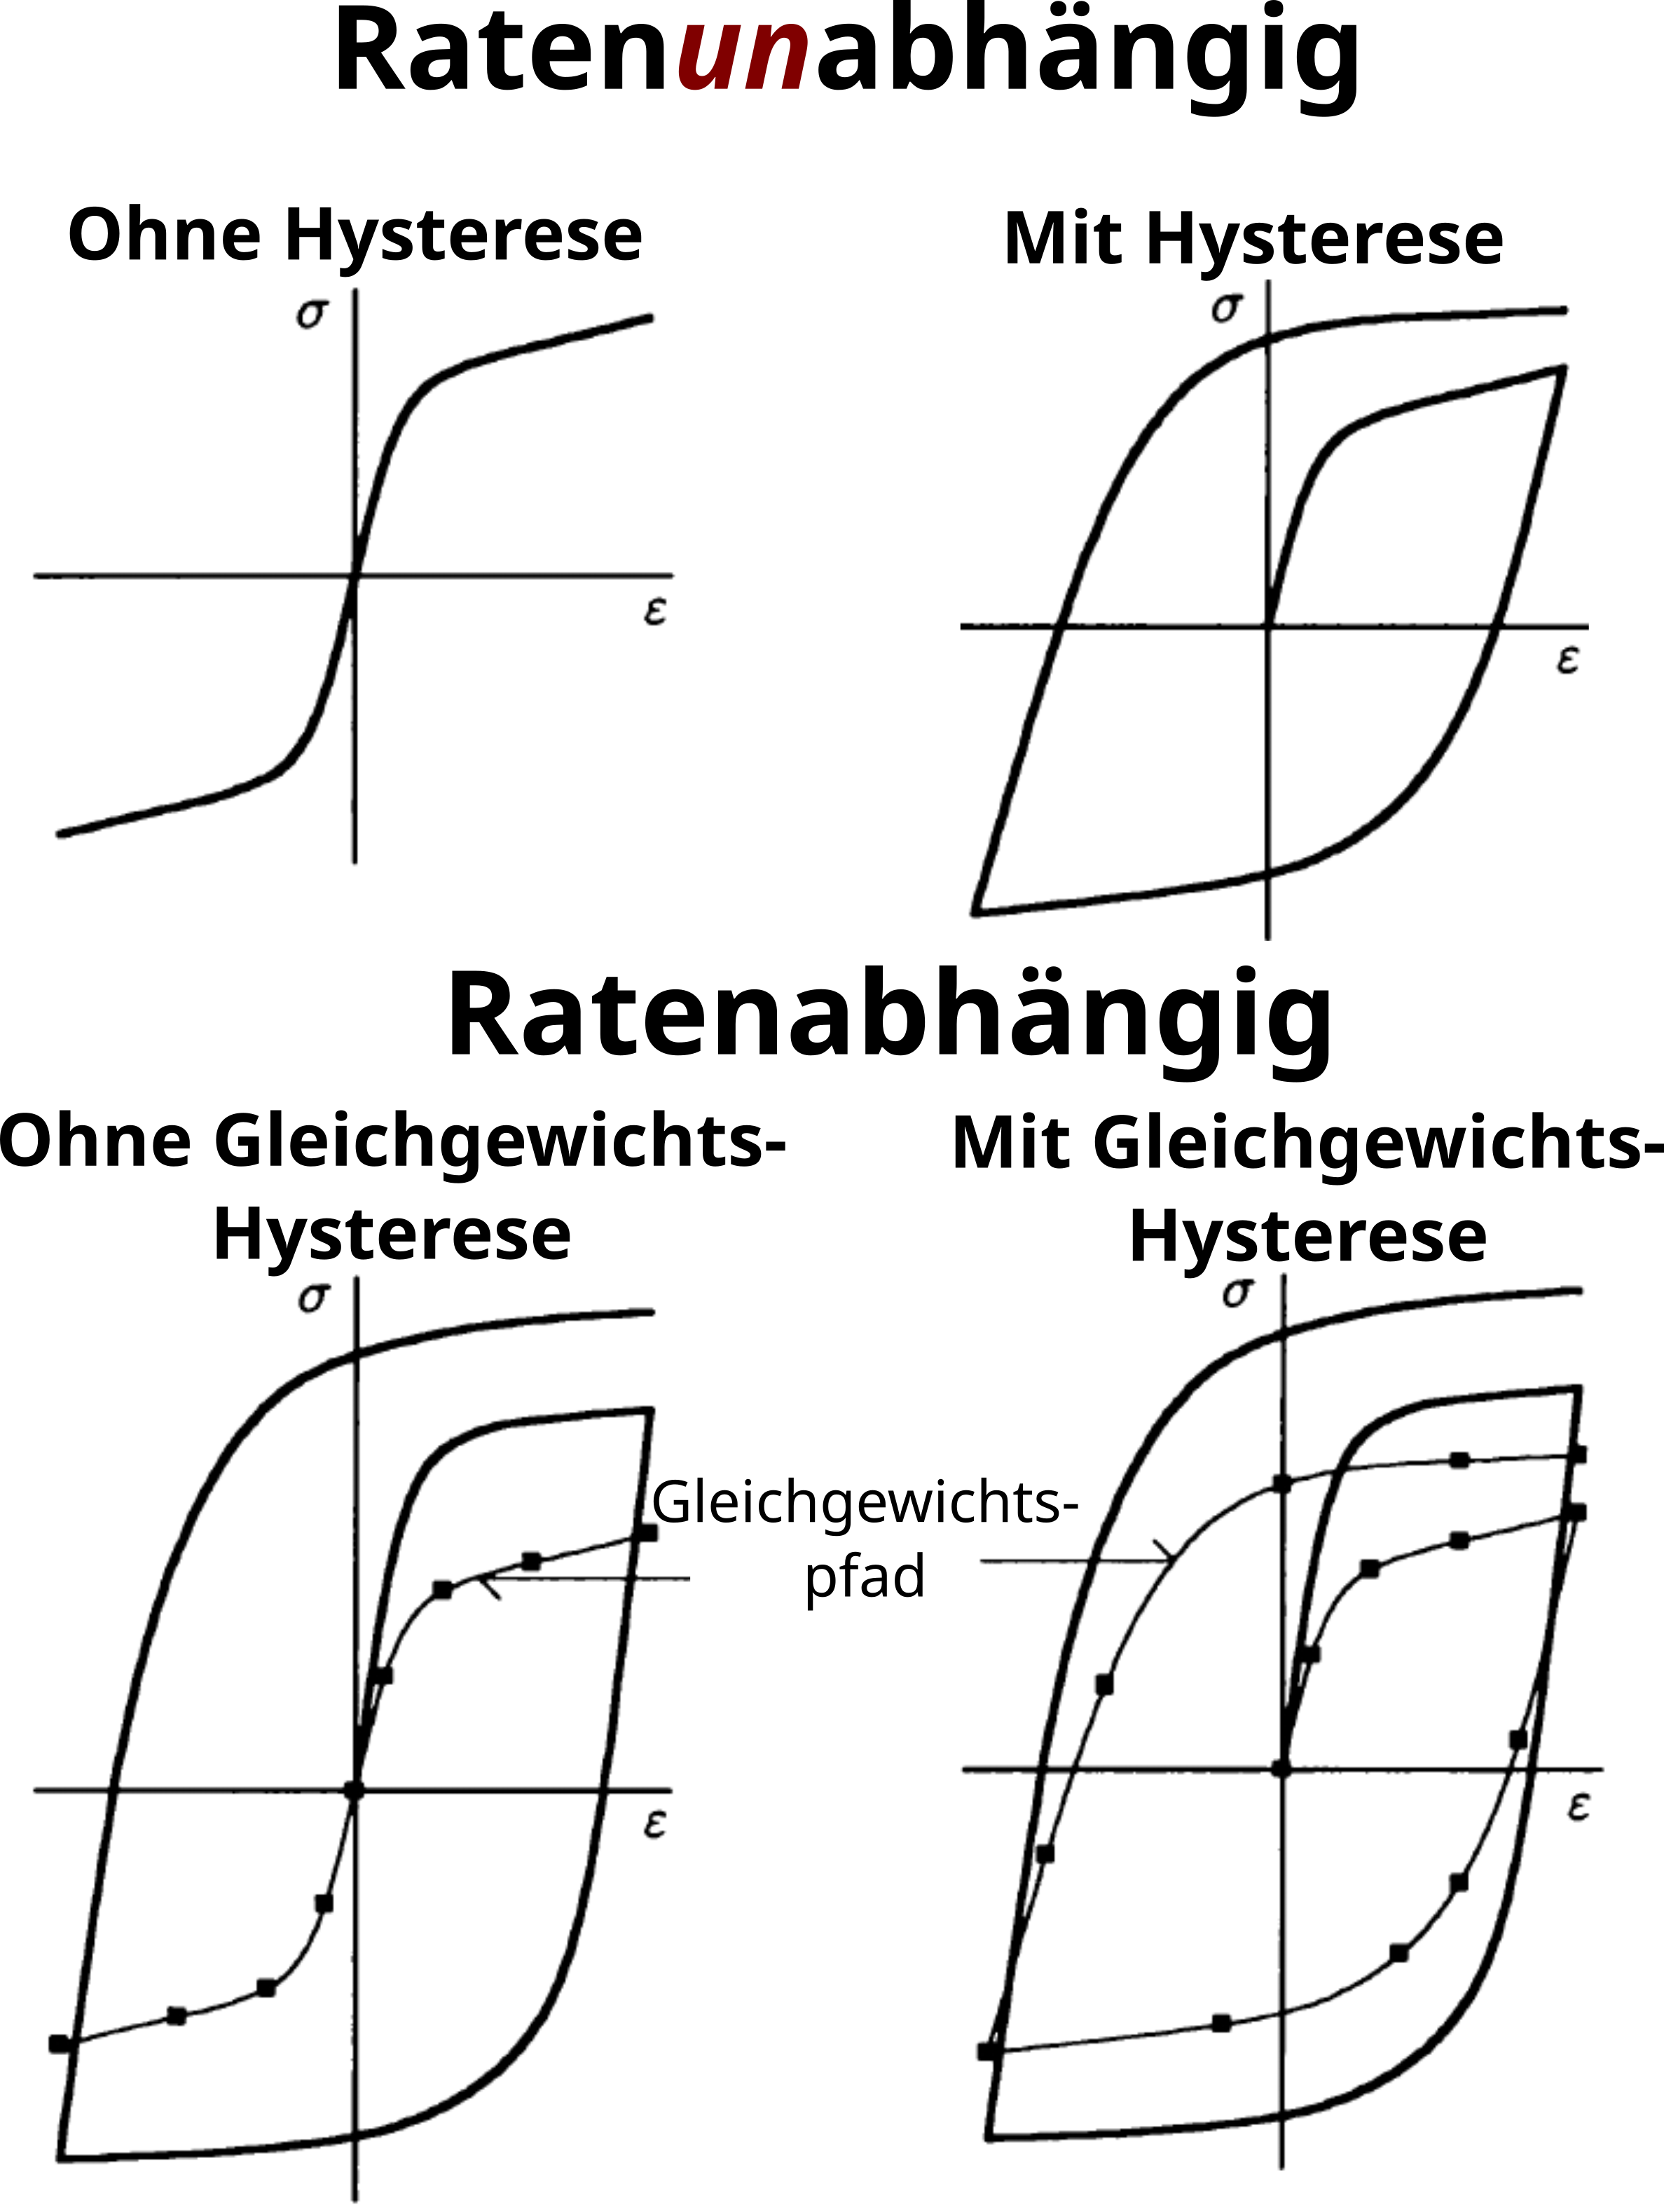
\includegraphics[width=0.7\linewidth]{files/Materialklassen-0654260d23db48934efafd3d240353a4.png}
\caption[]{Klassifizierung von Materialmodellen anhand ihrer Systemantwort. Abbildung nach \cite{haupt2013continuum}}
\label{materialklassen}
\end{figure}

%  -+-+-+-+-+-+-AI-SPLIT

\subparagraph{Wärmeleitung}

Bei der Berechnung der Wärmeleitungsgleichung wird oftmals die \textbf{Fourier}sche Wärmeleitung zugrunde gelegt. Diese basiert auf der Annahme, dass der Wärmestrom proportional zum negativen Temperaturgradienten ist:

\begin{equation}
\label{fourier}
\bm{q} = - \bm{k}\T  \grad{\theta} \, .
\end{equation}
Hierbei ist $\bm{k}$ der Konduktivitätstensor, welcher für isotrope Materialien wie folgt aussieht:
\begin{equation}
\label{konduktivitaetsmatrixIsotrop}
 \bm{k} = k \begin{bmatrix} 1 & 0 & 0 \\ 0 & 1 & 0 \\ 0 & 0 & 1\end{bmatrix}  \, ,
\end{equation}
mit der Wärmeleitfähigkeit $k$ in $\frac{\text{W}}{\text{m}\cdot\text{K}}$. Der Wärmestromvektor hat damit die Einheit $\frac{\text{W}}{\text{m}^2}$.

\begin{framed}
\textbf{Zusätzliche Gleichungen}\\
Aus Gleichung (\ref{fourier}) erhalten wir \textbf{3} zusätzliche Gleichungen. Wir haben jetzt genauso viele Gleichungen wie Unbekannte.
\end{framed}

\begin{framed}
\textbf{Materialsymmetrie (Auswahl)}\\
\begin{itemize}
\item isotrop - gleiche Eigenschaften in alle Raumrichtungen
\item transversal isotrop - unterschiedliche Eigenschaften entlang einer Faser (Symmetrieachse) und der zu dieser Faser senkrecht stehenden Ebene
\item orthotrop - drei paarweise senkrecht zueinander stehende Symmetrieachsen
\end{itemize}
\end{framed}

%  -+-+-+-+-+-+-AI-SPLIT

\subparagraph{Durchströmung}

Bei der Berechnung der Fluidgeschwindigkeit in Sickerströmungen wird oftmals das \textbf{Darcy}sche hydraulische Strömungsgesetz angewendet. Dies ist analog zur Wärmeleitung definiert als proportional zum negativen Druckgradienten:

\begin{equation}
\label{darcy}
\bm{v} = - \bm{k}_{\varepsilon}\T  \grad{p} \, .
\end{equation}
Hierbei ist $\bm{k}_{\varepsilon}$ die hydraulische Konduktivität. Für isotrope Materialien gilt:

\begin{equation}
 \bm{k}_{\varepsilon} = \frac{k_{\varepsilon}}{\mu} \begin{bmatrix} 1 & 0 & 0 \\ 0 & 1 & 0 \\ 0 & 0 & 1\end{bmatrix}  \, ,
\end{equation}
mit der hydraulischen Permeabilität $k_{\varepsilon}$ in $\text{m}^2$ und der dynamischen Viskosität $\mu$ in $\text{Pa}\cdot \text{s}$.

\begin{framed}
\textbf{Zusätzliche Gleichungen}\\
Aus Gleichung (\ref{darcy}) erhalten wir \textbf{3} zusätzliche Gleichungen. Wir haben jetzt genauso viele Gleichungen wie Unbekannte.
\end{framed}

%  -+-+-+-+-+-+-AI-SPLIT

\subparagraph{Lineare Elastizität}

In Figure~\ref{materialklassen} sind verschiedene Klassen von Festkörpermaterialien dargestellt. In dieser Vorlesung behandeln wir lediglich eine Unterklasse der ratenunabhängigen Materialien ohne Hysterese. Die lineare Elastizität ist gekennzeichnet durch einen linearen Zusammenhang zwischen Spannung $\bm{\sigma}$ und Dehnungen $\bm{\epsilon}$. In tensorieller Notation stellt sich das verallgemeinerte Hooke'sche Gesetz wie folgt dar:

\begin{equation}
\label{generalHook}
\sigma_{ij} = \mathbb{C}_{ijkl} \epsilon_{kl} \;
\end{equation}

wobei von der Einsteinschen Summenkonvention Gebrauch gemacht wurde. In der Strukturmechanik ist es jedoch unüblich, mit Tensoren 4. Stufe explizit zu rechnen. Es werden Symmetrieeigenschaften der Tensoren $\sigma_{ij}=\sigma_{ji}$, $\epsilon_{ij}=\epsilon_{ji}$ und $\mathbb{C}_{ijkl}=\mathbb{C}_{klij}$ ausgenutzt, um Tensorprodukte wie z.B. in Gleichung (\ref{generalHook}) in Matrix-Vektor-Operationen zu überführen. Dies ist vor allem für die numerische Implementierung von gro$\beta$em Vorteil.

\begin{equation}
\label{generalHook2}
\begin{bmatrix} 
\sigma_{11} \\
\sigma_{22} \\
\sigma_{33} \\
\sigma_{12} \\
\sigma_{23} \\
\sigma_{13} 
\end{bmatrix} = \begin{bmatrix}
C_{1111} & C_{1122} & C_{1133} & C_{1112} & C_{1123} & C_{1113} \\
C_{2211} & C_{2222} & C_{2233} & C_{2212} & C_{2223} & C_{2213} \\
C_{3311} & C_{3322} & C_{3333} & C_{3312} & C_{3323} & C_{3313} \\
C_{1211} & C_{1222} & C_{1233} & C_{1212} & C_{1223} & C_{1213} \\
C_{2311} & C_{2322} & C_{2333} & C_{2312} & C_{2323} & C_{2313} \\
C_{1311} & C_{1322} & C_{1333} & C_{1312} & C_{1323} & C_{1313} \\ 
\end{bmatrix} \begin{bmatrix} \epsilon_{11} \\ \epsilon_{22} \\ \epsilon_{33} \\ 2\epsilon_{12} \\ 2\epsilon_{23} \\ 2\epsilon_{13} \end{bmatrix}
\end{equation}

Für isotrope lineare Elastizität mit den Materialkonstanten:

\begin{itemize}
\item $E$ - Elastizitätsmodul in $\text{MPa}$
\item $\nu$ - Querkontraktionszahl in [-]
\end{itemize}

erhält man dann:

\begin{equation}
\label{generalHook3}
\begin{bmatrix} 
\sigma_{11} \\
\sigma_{22} \\
\sigma_{33} \\
\sigma_{12} \\
\sigma_{23} \\
\sigma_{13} 
\end{bmatrix} = \frac{E}{(1+\nu)(1-2\nu)}\begin{bmatrix}
1-\nu & \nu & \nu & 0 & 0 & 0 \\
\nu & 1-\nu & \nu & 0 & 0 & 0 \\
\nu & \nu & 1-\nu & 0 & 0 & 0 \\
0 & 0 & 0 & \frac{1-2\nu}{2} & 0 & 0 \\
0 & 0 & 0 & 0 & \frac{1-2\nu}{2} & 0 \\
0 & 0 & 0 & 0 & 0 & \frac{1-2\nu}{2} \\ 
\end{bmatrix} \begin{bmatrix} \epsilon_{11} \\ \epsilon_{22} \\ \epsilon_{33} \\ 2\epsilon_{12} \\ 2\epsilon_{23} \\ 2\epsilon_{13} \end{bmatrix}
\end{equation}

Für die inverse Beziehung $\bm{\epsilon} = \bm{C}^{ -1} \bm{\sigma}$ mit der Nachgiebigkeitsmatrix $\bm{C}^{ -1}$ erhält man:
\begin{equation}
\label{generalHook4}
\begin{bmatrix} 
\epsilon_{11} \\
\epsilon_{22} \\
\epsilon_{33} \\
2\epsilon_{12} \\
2\epsilon_{23} \\
2\epsilon_{13} 
\end{bmatrix} =\begin{bmatrix}
\frac{1}{E} & \frac{-\nu}{E} & \frac{-\nu}{E} & 0 & 0 & 0 \\
\frac{-\nu}{E} & \frac{1}{E} & \frac{-\nu}{E} & 0 & 0 & 0 \\
\frac{-\nu}{E} & \frac{-\nu}{E} & \frac{1}{E} & 0 & 0 & 0 \\
0 & 0 & 0 & \frac{1}{G} & 0 & 0 \\
0 & 0 & 0 & 0 & \frac{1}{G} & 0 \\
0 & 0 & 0 & 0 & 0 & \frac{1}{G} \\ 
\end{bmatrix} \begin{bmatrix} \sigma_{11} \\ \sigma_{22} \\ \sigma_{33} \\ \sigma_{12} \\ \sigma_{23} \\ \sigma_{13} \end{bmatrix}
\end{equation}

wobei $G=\frac{E}{2(1+\nu)}$ den Schubmodul in $\text{MPa}$ darstellt.

\begin{framed}
\textbf{Zusätzliche Gleichungen}\\
Aus Gleichung (\ref{generalHook3}) und (\ref{generalHook4}) erhalten wir \textbf{6} zusätzliche Gleichungen. Wir haben jetzt genauso viele Gleichungen wie Unbekannte.
\end{framed}

%  -+-+-+-+-+-+-AI-SPLIT

\begin{framed}
\textbf{Einsteinsche Summenkonvention}\\
Die Einsteinsche Summenkonvention ist eine Notationsvereinbarung, die in der Tensorrechnung verwendet wird, um Ausdrücke zu vereinfachen. Wenn ein Index in einem mathematischen Ausdruck zweimal vorkommt, wird implizit über diesen Index summiert:

\begin{equation}
c_i = \sum_{j=1}^{n} a_{ij} b_j \qquad \rightarrow \qquad  c_i=a_{ij} b_j
\end{equation}
\end{framed}

\begin{framed}
\textbf{Kelvin-Notation vs. Voigt-Notation}\\
Die Kelvin-Notation und die Voigt-Notation sind zwei verschiedene Methoden, um tensorielle Grö$\beta$en in Matrix- und Vektorschreibweise zu überführen. In den meisten kommerziellen FEM-Programmen ist die Voigt-Notation vorzufinden, wobei neuere FE-Codes durchaus die Vorteile der Kelvin-Notation ausnutzen \cite{nagel2016advantages}. Allgemein kann gesagt werden, dass die Voigt-Notation näher an der Ingenieurmechanik ist, da die Scheranteile $\epsilon_{ij} \quad \forall i\neq j$ der Dehnung doppelt eingehen und wir somit die Gleitungen $\gamma_{ij} \quad \forall i\neq j$ erhalten. Die Kelvin-Notation hat den Vorteil, dass mit ihr weiterhin alle Tensorprodukte einfach gebildet werden können, ohne dass über den Vorfaktor der Komponenten nachgedacht werden muss. Im aktuellen Kurs wird die \textbf{Voigt}-Notation zugrunde gelegt.

\bigskip\noindent
\begin{tabular}{p{\dimexpr 0.500\linewidth-2\tabcolsep}p{\dimexpr 0.500\linewidth-2\tabcolsep}}
\toprule
 & Voigt-Notation \\
\hline
$\sigma_{ij}$ & $\bm{\sigma}= \begin{bmatrix} \sigma_{11} & \sigma_{22} & \sigma_{33} & \sigma_{12} & \sigma_{23} & \sigma_{13} \end{bmatrix}\T$ \\
$\epsilon_{ij}$ & $\bm{\epsilon}= \begin{bmatrix} \epsilon_{11} & \epsilon_{22} & \epsilon_{33} & 2\epsilon_{12} & 2\epsilon_{23} & 2\epsilon_{13} \end{bmatrix}\T$ \\
$\sigma_{ij}=\mathbb{C}_{ijkl}\epsilon_{kl}$ & $\bm{\sigma} = \bm{C} \bm{\epsilon}$ \\
$\mathcal{E}=\sigma_{ij}\epsilon_{ij}$ & $\mathcal{E} = \bm{\sigma}\T\bm{\epsilon}$ \\
\bottomrule
\end{tabular}

\bigskip\begin{equation}
\mathbb{C}_{ijkl} \quad \rightarrow \quad \bm{C}=\begin{bmatrix}
C_{1111} & C_{1122} & C_{1133} & C_{1112} & C_{1123} & C_{1113} \\
C_{2211} & C_{2222} & C_{2233} & C_{2212} & C_{2223} & C_{2213} \\
C_{3311} & C_{3322} & C_{3333} & C_{3312} & C_{3323} & C_{3313} \\
C_{1211} & C_{1222} & C_{1233} & C_{1212} & C_{1223} & C_{1213} \\
C_{2311} & C_{2322} & C_{2333} & C_{2312} & C_{2323} & C_{2313} \\
C_{1311} & C_{1322} & C_{1333} & C_{1312} & C_{1323} & C_{1313} \\ 
\end{bmatrix}
\end{equation}

\bigskip\noindent
\begin{tabular}{p{\dimexpr 0.500\linewidth-2\tabcolsep}p{\dimexpr 0.500\linewidth-2\tabcolsep}}
\toprule
 & Kelvin-Notation \\
\hline
$\sigma_{ij}$ & $\bm{\sigma}= \begin{bmatrix} \sigma_{11} & \sigma_{22} & \sigma_{33} & \sqrt{2}\sigma_{12} & \sqrt{2}\sigma_{23} & \sqrt{2}\sigma_{13} \end{bmatrix}\T$ \\
$\epsilon_{ij}$ & $\bm{\epsilon}= \begin{bmatrix} \epsilon_{11} & \epsilon_{22} & \epsilon_{33} & \sqrt{2}\epsilon_{12} & \sqrt{2}\epsilon_{23} & \sqrt{2}\epsilon_{13} \end{bmatrix}\T$ \\
$\sigma_{ij}=\mathbb{C}_{ijkl}\epsilon_{kl}$ & $\bm{\sigma} = \bm{C} \bm{\epsilon}$ \\
$\mathcal{E}=\sigma_{ij}\epsilon_{ij}$ & $\mathcal{E} = \bm{\sigma}\T\bm{\epsilon}$ \\
\bottomrule
\end{tabular}

\bigskip\begin{equation}
\mathbb{C}_{ijkl} \quad \rightarrow \quad \bm{C}=\begin{bmatrix}
C_{1111} & C_{1122} & C_{1133} & \sqrt{2}C_{1112} & \sqrt{2}C_{1123} & \sqrt{2}C_{1113} \\
C_{2211} & C_{2222} & C_{2233} & \sqrt{2}C_{2212} & \sqrt{2}C_{2223} & \sqrt{2}C_{2213} \\
C_{3311} & C_{3322} & C_{3333} & \sqrt{2}C_{3312} & \sqrt{2}C_{3323} & \sqrt{2}C_{3313} \\
\sqrt{2}C_{1211} & \sqrt{2}C_{1222} & \sqrt{2}C_{1233} & 2C_{1212} & 2C_{1223} & 2C_{1213} \\
\sqrt{2}C_{2311} & \sqrt{2}C_{2322} & \sqrt{2}C_{2333} & 2C_{2312} & 2C_{2323} & 2C_{2313} \\
\sqrt{2}C_{1311} & \sqrt{2}C_{1322} & \sqrt{2}C_{1333} & 2C_{1312} & 2C_{1323} & 2C_{1313} \\ 
\end{bmatrix}
\end{equation}
\end{framed}

%  -+-+-+-+-+-+-AI-SPLIT

\subparagraph{Ebener Verzerrungszustand}

\begin{figure}[!htbp]
\centering
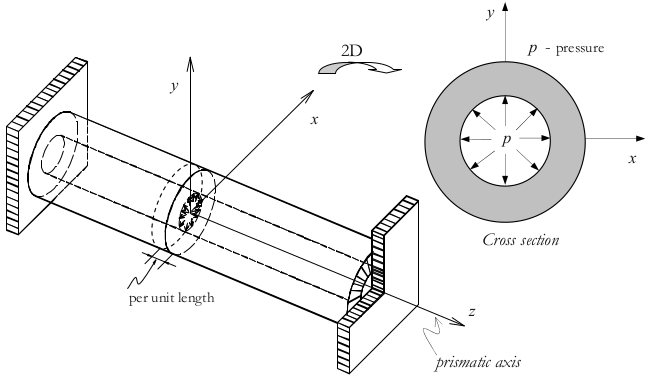
\includegraphics[width=0.7\linewidth]{files/EVZ-d6cb9ec161125a880d46ccc9573e94fb.png}
\caption[]{Beispiel für das Auftreten eines ebenen Verzerrungszustands \cite{chaves2013notes}}
\label{evz}
\end{figure}

Betrachten wir ein Strukturelement mit prismatischen Merkmalen, bei dem die Dimension in Richtung der prismatischen Achse deutlich grö$\beta$er ist als die anderen Dimensionen. Die aufgebrachten Lasten wirken senkrecht zur prismatischen Achse (Figure~\ref{evz}). Unter diesen Bedingungen sind die Dehnungskomponenten $\e_{13},\, \e_{23}, \, \e_{33}$ gleich null. Dieser Zustand wird als ebener Verzerrungszustand bezeichnet. Beispiele hierfür sind Stützmauern, unter Druck stehende Zylinder, Dämme, Tunnel und Flachgründungen.

Es muss betont werden, dass die Variablen (Last, Querschnitt, Material) entlang der prismatischen Achse konstant sein müssen, um einen ebenen Verzerrungszustand zu betrachten. Andernfalls können erhebliche Fehler auftreten.

\begin{framed}
\textbf{Prismatische Merkmale}\\
\begin{itemize}
\item Konstanter Querschnitt entlang der Längsachse
\item Längliche Form
\item Geradlinige Achse
\end{itemize}

\textbf{Beispiele:} Balken, Säulen, Rohre
\end{framed}

Um die konstitutive Beziehung $\sb(\eb)$ zu erhalten, starten wir vom generalisierten Hook'schen Gesetz (\ref{generalHook3}), indem wir alle Spalten mit korrespondierenden 0-Dehnungen eliminieren:

\begin{equation}
\label{evz1}
\begin{bmatrix} 
\sigma_{11} \\
\sigma_{22} \\
\sigma_{33} \\
\sigma_{12} \\
\sigma_{23} \\
\sigma_{13} 
\end{bmatrix} = \frac{E}{(1+\nu)(1-2\nu)}\begin{bmatrix}
1-\nu & \nu & \cancel{\nu} & 0 & \cancel{0} & \cancel{0} \\
\nu & 1-\nu & \cancel{\nu} & 0 & \cancel{0} & \cancel{0} \\
\nu & \nu & \cancel{1-\nu} & 0 & \cancel{0} & \cancel{0} \\
0 & 0 & \cancel{0} & \frac{1-2\nu}{2} & \cancel{0} & \cancel{0} \\
0 & 0 & \cancel{0} & 0 & \cancel{\frac{1-2\nu}{2}} & \cancel{0} \\
0 & 0 & \cancel{0} & 0 & \cancel{0} & \cancel{\frac{1-2\nu}{2}} \\ 
\end{bmatrix} \begin{bmatrix} \epsilon_{11} \\ \epsilon_{22} \\ \cancel{\epsilon_{33}} \\ 2\epsilon_{12} \\ \cancel{2\epsilon_{23}} \\ \cancel{2\epsilon_{13}} \end{bmatrix}
\end{equation}

Wir sehen sofort, dass die Komponenten $\s_{23},\, \s_{13}$ verschwinden. Die Spannungskomponente entlang der prismatischen Achse $\s_{33}$ hingegen berechnet sich zu:

\begin{equation}
\s_{33} = \frac{E \nu}{(1+\nu)(1-2\nu)} \left(\e_{11} + \e_{22} \right)
\end{equation}

%  -+-+-+-+-+-+-AI-SPLIT

Arrangiert man die verbleibenden Einträge, so erhält man für $\bm{C}\rs{EVZ}$:
\begin{equation}
\label{evz2}
 \begin{bmatrix} 
\s_{11} \\
\s_{22} \\
\s_{12} 
\end{bmatrix}= \underbrace{\frac{E }{(1+\nu)(1-2\nu)} \begin{bmatrix}
1-\nu & \nu & 0 \\
\nu & 1-\nu & 0 \\
0 & 0 & \frac{1-2\nu}{2}
\end{bmatrix}}_{\bm{C}\rs{EVZ}}  \begin{bmatrix} 
\e_{11} \\
\e_{22} \\
\e_{12} 
\end{bmatrix}
\end{equation}

Für die Nachgiebigkeit $\bm{C}\rs{EVZ}^{ -1}$ erhält man die inverse Beziehung:
\begin{equation}
\label{evz3}
 \begin{bmatrix} 
\e_{11} \\
\e_{22} \\
\e_{12} 
\end{bmatrix}= \underbrace{\frac{1+\nu }{E} \begin{bmatrix}
1-\nu & -\nu & 0 \\
-\nu & 1-\nu & 0 \\
0 & 0 & 2
\end{bmatrix}}_{\bm{C}\rs{EVZ}^{-1}}  \begin{bmatrix} 
\s_{11} \\
\s_{22} \\
\s_{12} 
\end{bmatrix}
\end{equation}

%  -+-+-+-+-+-+-AI-SPLIT

\subparagraph{Ebener Spannungszustand}

\begin{figure}[!htbp]
\centering
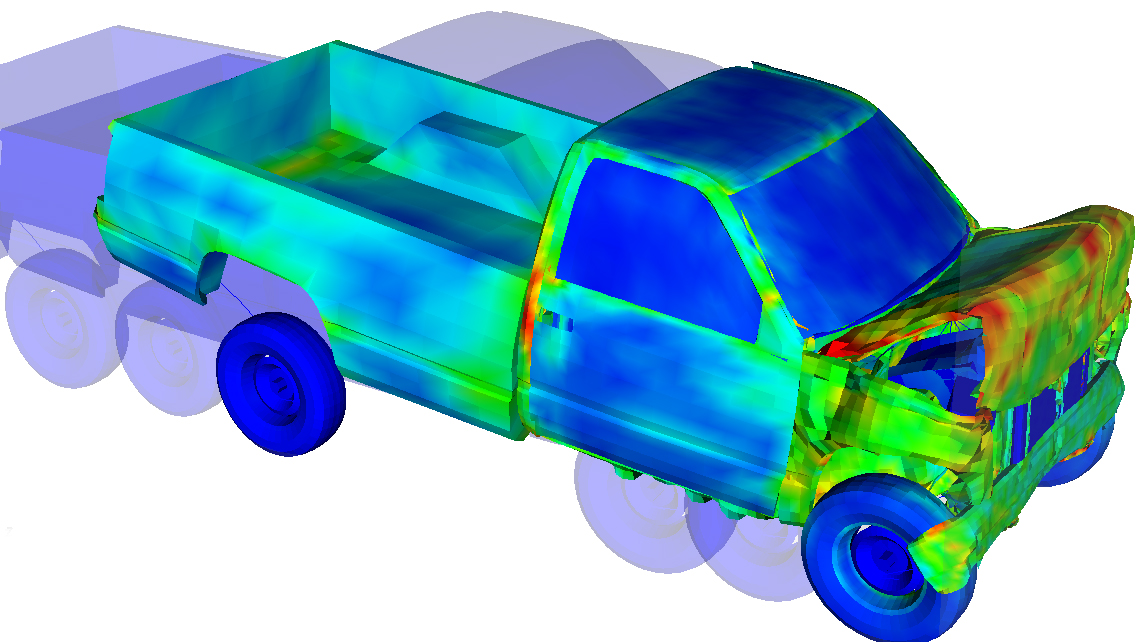
\includegraphics[width=0.7\linewidth]{files/CarCrash-dbcc46180747582567a8cdb800f7cc04.jpg}
\caption[]{FEM Crash-Simulation eines Pickup-Trucks gegen eine starre Wand \href{https://enteknograte.com/wp-content/uploads/2022/06/truck-crash-Car-vehicle-Finite-Element-Simulation-Crash-Test-MSC-dytran-Crashworthiness-Ls-Dyna-Abaqus-PAM-CRASH.jpg}{Quelle}}
\label{carcrash}
\end{figure}

Der ebene Spannungszustand tritt überall dort auf, wo Flächenelemente vor allem in ihrer Ebene belastet werden und die Flächenabmessungen deutlich grö$\beta$er sind als die dazugehörige Dicke. Dies ist zum Beispiel bei Karosserieblechen, wie in Figure~\ref{carcrash}, der Fall.

\begin{figure}[!htbp]
\centering
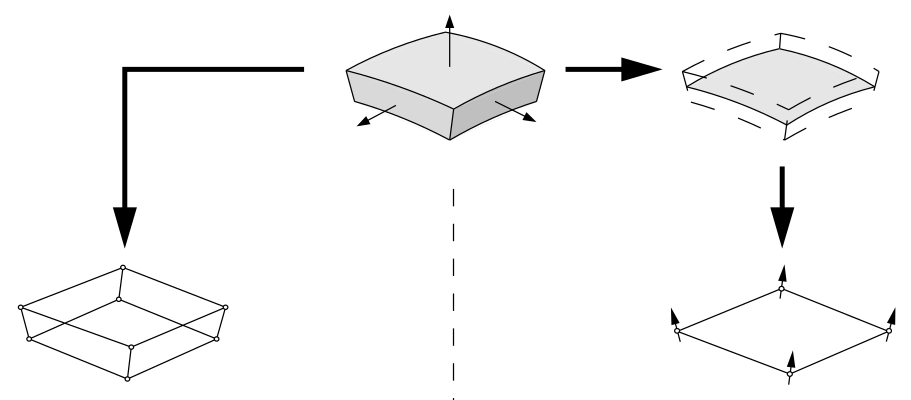
\includegraphics[width=0.7\linewidth]{files/Shellformulation-69f62cd7489fe0ebc779931fdd28af92.png}
\caption[]{FEM-Diskretisierung von Schalenelementen als degenerierte Volumenelemente (links) oder über eine Mittelflächendarstellung (rechts). \cite{wriggers2008nonlinear}}
\label{shellformulation}
\end{figure}

In Abbildung Figure~\ref{shellformulation} auf der rechten Seite ist eine Diskretisierung für den ebenen Spannungszustand mit Mittelflächenelementen zu sehen.

Startpunkt für die konstitutive Beziehung ist die Gleichung (\ref{generalHook4}). Zunächst streichen wir alle Spalten, die den 0-Spannungen zugeordnet werden können:
\begin{equation}
\label{generalHookESZ1}
\begin{bmatrix} 
\epsilon_{11} \\
\epsilon_{22} \\
\epsilon_{33} \\
2\epsilon_{12} \\
2\epsilon_{23} \\
2\epsilon_{13} 
\end{bmatrix} = \begin{bmatrix}
\frac{1}{E} & \frac{-\nu}{E} & \cancel{\frac{-\nu}{E}} & 0 & \cancel{0} & \cancel{0} \\
\frac{-\nu}{E} & \frac{1}{E} & \cancel{\frac{-\nu}{E}} & 0 & \cancel{0} & \cancel{0} \\
{\frac{-\nu}{E}} & {\frac{-\nu}{E}} & \cancel{\frac{1}{E}} & {0} & \cancel{0} & \cancel{0} \\
0 & 0 & \cancel{0} & \frac{1}{G} & 0 & 0 \\
{0} & {0} & \cancel{0} & {0} & \cancel{\frac{1}{G}} & \cancel{0} \\
{0} & {0} & \cancel{0} & {0} & \cancel{0} & \cancel{\frac{1}{G}} \\ 
\end{bmatrix} \begin{bmatrix} \sigma_{11} \\ \sigma_{22} \\ \cancel{\sigma_{33}} \\ \sigma_{12} \\ \cancel{\sigma_{23}} \\ \cancel{\sigma_{13}} \end{bmatrix}
\end{equation}

Hier fällt auf, dass das resultierende System nicht mehr quadratisch ist, da die Dehnung in Dickenrichtung $\epsilon_{33}$ ungleich null ist:

\begin{equation}
\label{generalHookESZ2}
\begin{bmatrix} 
\epsilon_{11} \\
\epsilon_{22} \\
\epsilon_{33} \\
2\epsilon_{12} \\
\end{bmatrix} = \begin{bmatrix}
\frac{1}{E} & \frac{-\nu}{E}  & 0  \\
\frac{-\nu}{E} & \frac{1}{E}  & 0  \\
{\frac{-\nu}{E}} & {\frac{-\nu}{E}} & {0} \\
0 & 0 & \frac{1}{G}  \\
\end{bmatrix} \begin{bmatrix} \sigma_{11} \\ \sigma_{22} \\ \sigma_{12} \end{bmatrix} \; .
\end{equation}

Dieses System hat eine Gleichung zu viel. Zweckmä$\beta$ig vernachlässigt man die Gleichung für die Dehnung in Dickenrichtung (diese Dehnung berechnet man in einer Nachlaufrechnung). Somit lautet die Nachgiebigkeitsmatrix $\bm{C}^{ -1}\rs{ESZ}$ und die materielle Steifigkeitsmatrix $\bm{C}\rs{ESZ}$ für den ebenen Spannungszustand:

\begin{equation}
\label{generalHookESZ3}
\bm{C}^{-1} = \frac{1}{E} \begin{bmatrix}
1 & -\nu & 0  \\
-\nu & 1  & 0  \\
0 & 0 & 2(1+\nu)  \\
\end{bmatrix}  \qquad 
\bm{C} = \frac{E}{(1-\nu^2)}\begin{bmatrix}
1 & \nu  & 0  \\
\nu & 1  & 0  \\
0 & 0 & \frac{1-\nu}{2}  \\
\end{bmatrix}
\end{equation}

%  -+-+-+-+-+-+-AI-SPLIT

\subparagraph{Rotationssymmetrie}

\begin{figure}[!htbp]
\centering
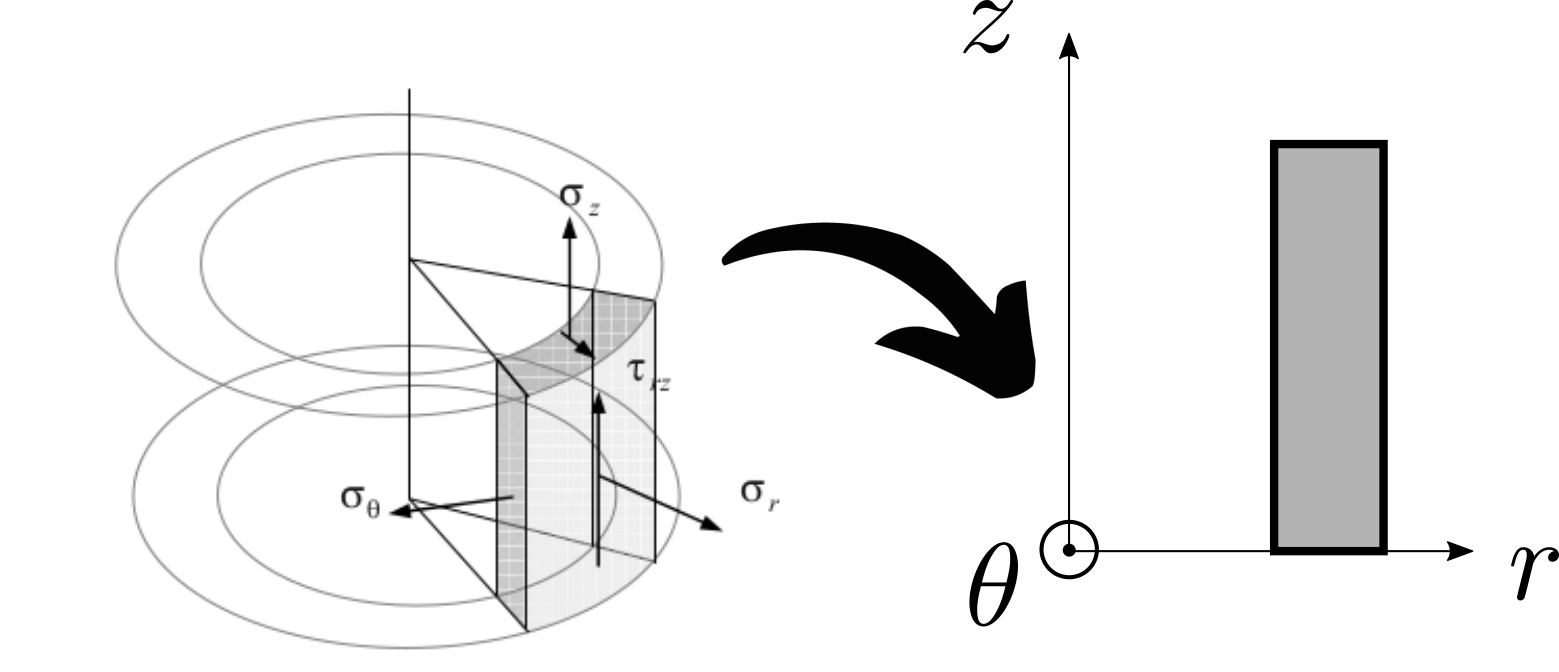
\includegraphics[width=0.7\linewidth]{files/Rotsym-3fba0d8dbcd585e051159d15272d95e0.png}
\caption[]{Rotationssymmetrischer Körper im Zylinderkoordinatensystem $\{r,z,\theta\}$. Nach \cite{chaves2013notes}}
\label{rotsym}
\end{figure}

Die Dehnungen für rotationssymmetrische Problemstellungen werden berechnet zu:

\begin{equation}
\label{rotsymstrain}
\begin{bmatrix}
\e_{r} \\
\e_z \\
\e_{\theta} \\
\gamma_{rz}
\end{bmatrix} = \begin{bmatrix}
\Pd{u}{r} \\
\Pd{v}{z} \\
\frac{u}{r} \\
\Pd{u}{z} + \Pd{v}{r}
\end{bmatrix}
\end{equation}

Das generalisierte Hooke'sche Gesetz lautet:

\begin{equation}
\label{generalHookRotsym}
\begin{bmatrix} 
\sigma_{rr} \\
\sigma_{zz} \\
\sigma_{\theta} \\
\sigma_{rz} \\
\end{bmatrix} = \frac{E}{(1+\nu)(1-2\nu)}\begin{bmatrix}
1-\nu & \nu & \nu & 0  \\
\nu & 1-\nu & \nu & 0  \\
\nu & \nu & 1-\nu & 0  \\
0 & 0 & 0 & \frac{1-2\nu}{2} \\
\end{bmatrix} \begin{bmatrix} \epsilon_{r} \\ \epsilon_{\theta} \\ \epsilon_{z} \\ 2\epsilon_{rz}  \end{bmatrix}
\end{equation}

\begin{framed}
\textbf{Berechnung der Dehnung $\e_{\theta}$}\\
Die Dehnung in Umfangsrichtung kann bestimmt werden als Längenänderung des Umfangs infolge einer radialen Verschiebung $u$:

$\e_{\theta} = \frac{2 \pi (r+u) -2\pi r}{2\pi r} = \frac{u}{r}$
\end{framed}

\paragraph{Zusammenfassung}

Um ein valides mechanisches Modell zu erlangen, benötigt man:

\begin{enumerate}
\item Die beschreibende partielle Differentialgleichung (physikalische Erhaltungssätze)
\item Die kinematischen Beziehungen (Verbindung von primärer Grö$\beta$e zur abgeleiteten Grö$\beta$e)
\item Materialmodell (Verbindung von sekundärer Grö$\beta$e zur kinematischen Grö$\beta$e)
\end{enumerate}

Eindeutig lösbar wird das Modell zudem erst, wenn die Randbedingungen entsprechend vorgegeben sind.

\begin{framed}
\textbf{Fragen zum Kapitel}\\
\textbf{Feldgleichungen der Kontinuumsmechanik}

\begin{itemize}
\item Nennen Sie die für die Strukturmechanik wesentliche Feldgleichung.


\item Nennen Sie drei verschiedene Feldgleichungen.


\item Welche Feldgrö$\beta$e wird mit der Impulsbilanz berechnet?


\item Welche Feldgrö$\beta$e wird mit der Energiebilanz berechnet?


\item Welche Feldgrö$\beta$e wird mit der Massenbilanz berechnet?


\item Was ist der Unterschied zwischen primären und sekundären Feldgrö$\beta$en?


\item Welche Aussage ist richtig:

\begin{itemize}
\item Die Impulsbilanz ist eine vektorielle partielle Differenzialgleichung.
\item Die Energiebilanz ist eine vektorielle partielle Differenzialgleichung.
\item Die sekundäre Feldgrö$\beta$e der Energiebilanz ist der Wärmefluss.
\item Die Massenbilanz ist für gewöhnliche Festkörper stets erfüllt und muss nicht separat gelöst werden.
\item Die Bilanzgleichungen sind materialunabhängige physikalische Prinzipien.
\item Zur Lösung der Bilanzgleichungen benötigt man noch weitere Restriktionen.
\end{itemize}


\item Welche Arten von Randbedingungen werden in der Mechanik von Festkörpern unterschieden?


\item Ist eine Kraftrandbedingung eine \textit{Neumann}-Randbedingung oder eine \textit{Dirichlet}-Randbedingung?


\item Ist eine Verschiebungsrandbedingung eine \textit{Neumann}-Randbedingung oder eine \textit{Dirichlet}-Randbedingung?
\end{itemize}

%  -+-+-+-+-+-+-AI-SPLIT

\textbf{Kinematik}

\begin{itemize}
\item Welche Aussage ist richtig:\begin{itemize}
\item Die Dehnung ist der symmetrische Anteil des Verschiebungsgradienten.
\item Die Spannung ist der symmetrische Anteil des Verschiebungsgradienten.
\item Die Ingenieursdehnungen sollten nur in einem Dehnungsbereich von \textless  10 \% eingesetzt werden.
\item Starrkörperrotationen rufen keine Ingenieurdehnungen (und auch keine Spannungen) hervor.
\end{itemize}
\end{itemize}

\textbf{Materialgleichung}

\begin{itemize}
\item Warum brauchen wir Materialgleichungen? (2 Gründe nennen)
\item Nennen Sie eine Klasse von Materialien entsprechend ihres Materialverhaltens für strukturmechanische Problemstellungen.
\item In welche Richtung flie$\beta$t die Temperatur bei der Fourierschen Wärmeleitung?
\item Was bedeutet isotropes Materialverhalten?
\item Wie viele Materialparameter sind nötig, um das Verhalten von linearen, isotropen und elastischen Materialien zu beschreiben?
\item Liegt bei Karosserieteilen eher ein ebener Spannungs- oder ein ebener Verzerrungszustand vor?
\end{itemize}

\textbf{Zusammenfassung}

\begin{itemize}
\item Welche 3 Dinge sind erforderlich, um ein lösbares mechanisches Modell zu erhalten?
\item Was ist zusätzlich notwendig, um eine eindeutige Lösung zu erhalten?
\end{itemize}

%  -+-+-+-+-+-+-AI-SPLIT
\end{framed}